\chapter{Background of Electrochemical Reprocessing} \label{ch:background}

The United States currently has approximately 70000 MTU of spent nuclear fuel (SNF) sitting either in intermediate length storage via spent fuel casks (heavily shielded concrete containers), or in spent fuel pools [insert CURIE citation here]. Most reactor sites are at or near their limit for pool storage, and above ground cask storage is becoming commonplace. The United States has responsibility for commercially produced spent nuclear fuel, per 10 CFR 961.11, listed below [insert 10 CFR citation]. \\

\begin{lstlisting}
Witnesseth that:

Whereas, the DOE has the responsibility for the disposal of spent nuclear fuel and high-level radioactive waste of domestic origin from civilian nuclear power reactors in order to protect the public health and safety, and the environment; and

Whereas, the DOE has the responsibility, following commencement of operation of a repository, to take title to the spent nuclear fuel or high-level radioactive waste involved as expeditiously as practicable upon the request of the generator or owner of such waste or spent nuclear fuel; and

Whereas, all costs associated with the preparation, transportation, and the disposal of spent nuclear fuel and high-level radioactive waste from civilian nuclear power reactors shall be borne by the owners and generators of such fuel and waste; and

Whereas, the DOE is required to collect a full cost recovery fee from owners and generators delivering to the DOE such spent nuclear fuel and/or high level radioactive waste; and

Whereas, the DOE is authorized to enter into contracts for the permanent disposal of spent nuclear fuel and/or high-level radioactive waste of domestic origin in DOE facilities; and

Whereas, the Purchaser desires to obtain disposal services from DOE; and

Whereas, DOE is obligated and willing to provide such disposal services, under the terms and conditions hereinafter set forth; and

Whereas, this contract is made and entered into under the authority of the DOE Organization Act ( Pub. L. 95-91, 42 U.S.C. 7101et seq.) and the Nuclear Waste Policy Act of 1982 ( Pub. L. 97-425, 42 U.S.C. 10101et seq.)

\end{lstlisting}

As such, the United States is currently investigating a number of possible solutions for spent nuclear fuel. The most widely known route is via direct disposal at a facility such as Yucca Mountain. This route would involve simply taking the spent fuel at reactor sites, repackaging it, and then disposing of it in a geologic repository. Some consider this route to be wasteful, not utilizing the full potential of nuclear fuel. The reason for this is that spent fuel is composed of $\approx 96\%$ uranium [insert world-nuclear citation], and reprocessing the SNF would offer multiple benefits. \\

\section{Reprocessing}
The first benefit is utilization of more of the potential energy of the nuclear fuel. Reprocessing the fuel allows the majority of the uranium to be used as fuel a second time, if also using fast spectrum reactors. A second benefit is the reduced amount of SNF, both in terms of total mass, and potentially, heat volume, that would be going to a repository. \\
\subsection{PUREX}
The United States has been reprocessing SNF since the Manhattan project, although not for the purpose of recycling commercial fuel. The United States has used the Plutonium Uranium Solvent Extraction (PUREX) process for decades to recover plutonium from specially burned nuclear fuel for the purpose of harvesting nuclear weapons material. This process involves multiple steps of reducing and oxidizing the uranium and plutonium, to produce an immiscible mixture, whereby uranium and plutonium are selectively extracted using compounds such as TBP to aid in extraction. This process is well understood, and there is significant experience with it. However, there are drawbacks. A significant amount of byproduct nuclear waste is produced via this method, and it can not be used on very fresh SNF, as there are heat limits to this technique. It is also not suitable to sodium bonded fuel [insert Argonne citation]. The last drawback is the large footprint required for a PUREX facility. \\
\subsection{Pyroprocessing}
An alternative method of reprocessing that has been proven to work is electrochemical reprocessing, also known as pyroprocessing. This method utilizes the fact that the Gibbs Free Energy of uranium, plutonium, and other transuranics have slight differences, and as such can be separated via adjusting the voltage going through a molten salt mixture. The process of pyroprocessing, of which the safeguards is the subject of this thesis, is described as follows. \\ % I don't like how this last sentence is worded.

\begin{figure}[h]
  \centering
  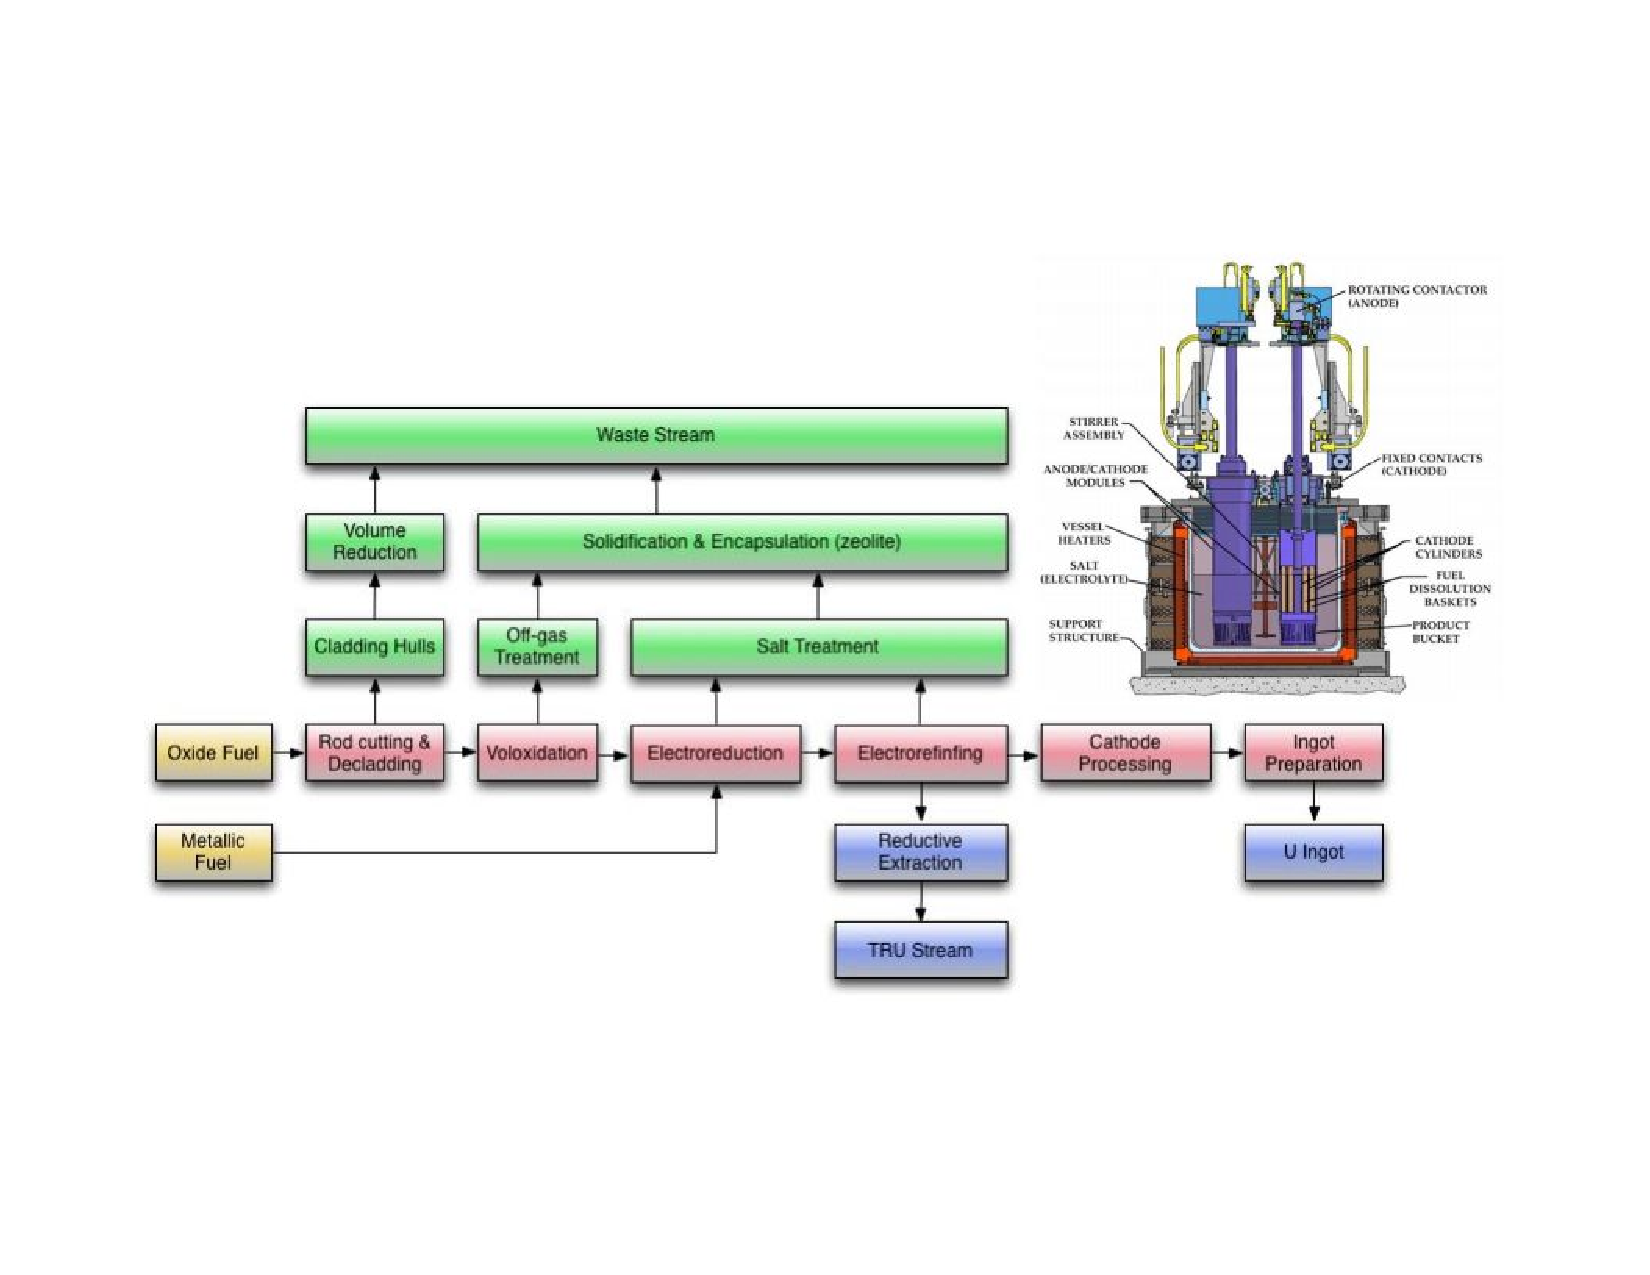
\includegraphics[width=15cm]{Pyroprocessing_Description_Skutnik.pdf}\\
  \caption{Flow sheet illustrating the pathways of pyroprocessing.}\label{pyro_flow}
\end{figure} 

\newpage

\subsection{Fuel Rod Processing}
As Figure \ref{pyro_flow} shows, the process starts with the spent fuel rods being extracted and then being chopped. The fuel pellets are then extracted, and sent to the voloxidizer, if it is not already in metallic form. The zirconium cladding fuel rod cladding is sent for metal waste disposal. This part is completely mechanical. The fuel pellets will then need to be oxidized via voloxidation. 

\subsection{Voloxidation}

Voloxidation serves two purposes: the first is to release and capture some of the fission gasses, and the second is to prepare the oxide fuel for electroreduction. Voloxidation is performed by flowing oxygen through a voloxidation reactor, producing the following reaction.

\begin{equation}
3UO_2 + O_2 \rightarrow U_3O_8
\end{equation}

The result of this is that the fuel material is converted to a less dense, higher surface area powder to be sent to electroreduction. Several items of note for this process are the air flow rate and the temperature of the system. The oxygen flow rate should be such that it produces the oxidizing reaction without being so high as to carry off fuel particles into the off gas stream. The temperature must be maintained above 500 $^{\circ}$C and below 1000 $^{\circ}$C. Temperatures above 1000 $^{\circ}$C can cause undesirable sintering of particles. An interesting item to note, is that the voloxidation process results in elimination of a fraction of the fission products. It eliminates the majority of the technetium and ruthenium, while elminating between $\frac{1}{5}$ to $\frac{1}{3}$ of the cesium.


\subsection{Electroreduction}

After the material has been pulverized and converted to $U_3O_8$, the material must then be electroreduced, to yield pure metalic material, rather than an oxide. The electrolyte used is $LiCl-Li_2O$ at 650 $^{\circ}$C, with a platinum rod anode. The cathode of this cell is the fuel powder, contained within a magnesia membrane walls, so ions can traverse the membrane to react. The reaction that takes place is shown below. \\ 

\begin{equation}
Li^+ + e^- \rightarrow Li
\end{equation}

\begin{equation}
M_xO_y + 2yLi \rightarrow xM + yLi_2O
\end{equation}

Some of the fission products such as cesium and barium (alkaline elements) will dissolve into the salt as metal chlorides, as it is electrochemically favorable for them to do so. These fission products can be disposed of when the salt is treated. The electroreduction process is extremely effective, reducing uranium and plutonium to metals at rates of $\approx$ 99 and 96 \%, respectively. The salt then has to be separated from the transuranic metals. This is done by evaporation at temperatures of around 1200 $^{\circ}$C. During this process, some actinides can be contained in the waste streams of fission products and salt. \\

\subsection{Electrorefiner}
 It is then inserted into a basket to be placed into the electrorefiner. At the electrorefiner, the fuel is dissolved into the molten salt with an applied voltage. The voltage applied will pull off components of the fuel in a particular order, corresponding to the Gibbs Free Energy. The lathanides will dissolve into the salt first, then the  uranium and transuranics will go into the salt. The noble metals (iron, zirconium, cadmium, etc) will stay in the chopped fuel basket, as they have higher Gibbs Free Energy. After uranium and transuranics are dissolved into the salt, the voltage is then lowered, allowing the reaction to proceed in reverse. The uranium will plate out first as dendrites on the solid cathode. After uranium collection on the solid cathode has saturated, the voltage is lowered again, this time pulling out the transuranics, along with some of the residual uranium, into a liquid cadmium cathode. After these two steps, the cathodes are sent off to collect the uranium and transuranics, eventually producing solid metal ingots. \\

The salt will over time accumulate fission products and trace amounts of uranium and transuranics. Every so often, the salt must be purified, with the fission products being captured in zeolite for storage/disposal. Throughout this process, whenever possible, off-gasses (such as tritium and xenon) are captured for disposal. \\

\section{Hybrid K-Edge Densitometry}

\subsection{Description of HKED}

Hybrid K-Edge densitometry is a nuclear safeguards technique that is based on two separate techniques k-edge densitometry (KED) and x-ray fluorescence (XRF), and combines them together into one measurement device. This technique has been proven to work for aqueous based reprocessing, and is scheduled to be used in the Rokkasho reprocessing facility in Japan [cite Rokkasho paper IAEA]. \\

K-edge densitometry works by using the fact that the mass attenuation coefficient for gamma rays encounters a significant increase around electron shells. In particular, the k-shell is of interest for several reasons. The first is that it is located at 115.6 keV, and is very noticeable. The second is that the mass attenuation coefficient for the k-edge is a very sharp, distinct rise and fall. These two factors combine to make for a very clean and easy measurement. \\

The k-edge drop occurs when a gamma ray passes through a material, such as molten salt, and encounters uranium. To perform this measurement, a gamma ray source is shown at a molten salt sample, with a detector behind the sample. Gamma rays interact more strongly with high atomic number material, so in the abscence of uranium, there is negligible gamma ray intensity drop at the 115.6 keV energy on a gamma detector. However, as uranium concentration in the salt is increased, a noticeable decrease in gamma ray intensity occurs around 115.6 keV in the detector pulse height spectrum. This is due to the uranium mass attenuation coefficient at 115.6 being significantly higher than the nearby energies, and blocking transmission of gammas at that energy. Plutonium's k-edge is located at 121.8 keV [cite los alamos].\\

X-ray fluorescence occurs as a result of the ejection of k-shell electrons due to photon interaction. This electron ejection causes a higher orbit electron to fall and take the vacant spot, emitting a characteristic x-ray. A list of common x-rays emitted from uranium and plutonium k-shell ejections is listed in \ref{xrays-uranium-plutonium} [cite Matt's Dissertation]. \\

\begin{table}[hb]
\caption{X-ray Energies Emitted By Uranium and Plutonium K-shell Ejections (keV)}
\label{xrays-uranium-plutonium}
\begin{center}
\begin{tabular}[b]{|c|c|c|c|c|c|c|}
	\hline
	Element & $K_{\alpha1}$ & $K_{\alpha2}$ & $K_{\beta1}$ & $K_{\beta2}$ & $K_{\beta3}$ & $K_{\beta4}$\\ \hline
	Uranium & 98.43 & 94.65 & 111.3 & 114.5 & 110.4 & 114.8 \\ \hline
	Plutonium & 103.7 & 99.52 & 117.2 & 120.6 & 116.2 & 120.9\\ \hline

\end{tabular}
\end{center}
\end{table}

Using a combination of these two techniques, it is possible to determine the concentration of elements such as actinides in the salt. 



